\xchapter{Proof of Concept: our model applied in different emergency scenarios}{}  \label{chapter:proofConcept}

 
As previously presented, our research was developed inside of the Rescuer project. In addition to producing knowledge on emergency management, the project also sought to propose intelligent solutions to help the emergency managers during a crisis. RESCUER News was born as our proposal for a smart solution to public communication of emergencies. 

Rescuer News was build based on our proposed model. The main challenge was to build a solution that could adapt to the multiple scenarios of an emergency, in particular for emergencies in industrial parks and large-scale events.

In this section, we present the Rescuer News configured for three different situations: emergency in an industrial park, in a stadium during a football match, and in a car accident inside a tunnel.


% \subsection{Posthof Linz Concert Hall simulation}

% \begin{figure*}[h]
% \centering
% \subfloat[Original]{
% 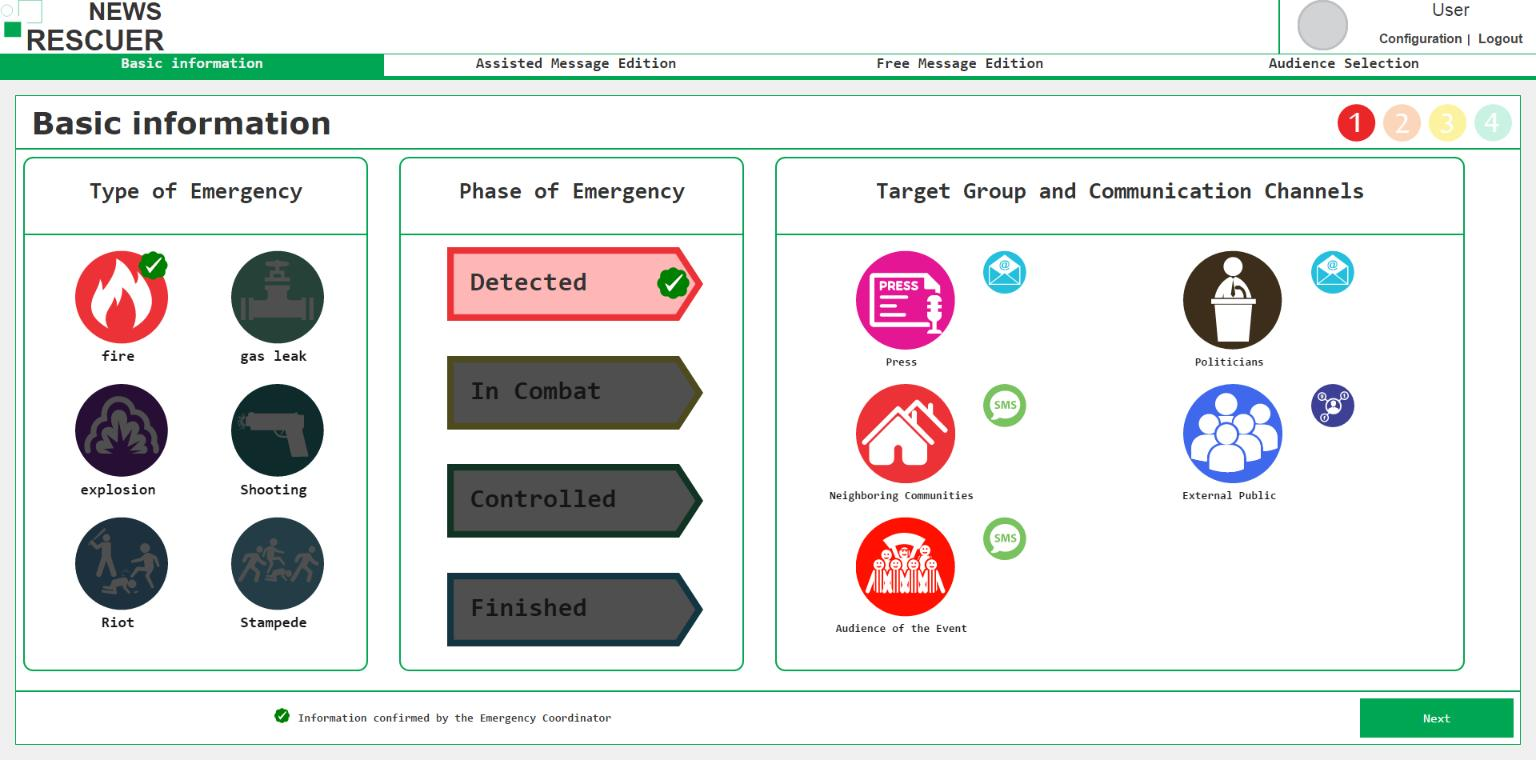
\includegraphics[width=0.46\linewidth]{images/DemoPosthof1.jpg}
% \label{demoPolo1}
% }
% \quad %espaco separador
% \subfloat[3x3]{
% 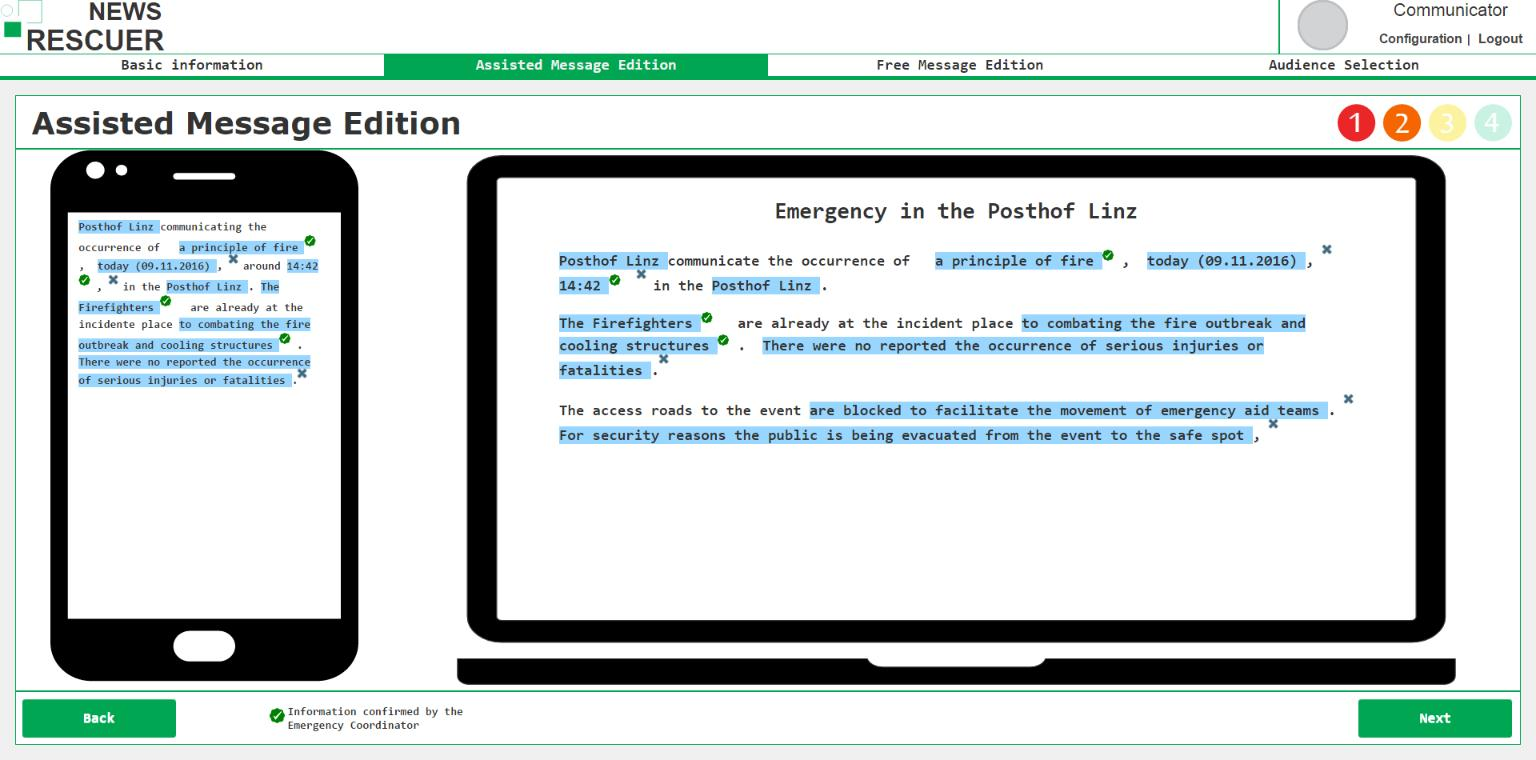
\includegraphics[width=0.46\linewidth]{images/DemoPosthof2.jpg}
% \label{demoPolo2}
% }
% \caption{RESCUER News configured for the Posthol Linz Concert Hall simulation}
% \label{fig02}
% \end{figure*}


\section{Demonstration at Stadion der Stadt Linz}

This demonstration was conducted at Stadion der Stadt Linz, Austria during a soccer game with an audience of around 800 people. In addition to the visitors, 36 security staff members, 15 policemen, and 15 first aid members worked in the event. 

\begin{figure*}[!h]
\centering
\subfloat[Basic information screen configured to the Demonstration at Stadion der Stadt Linz]{
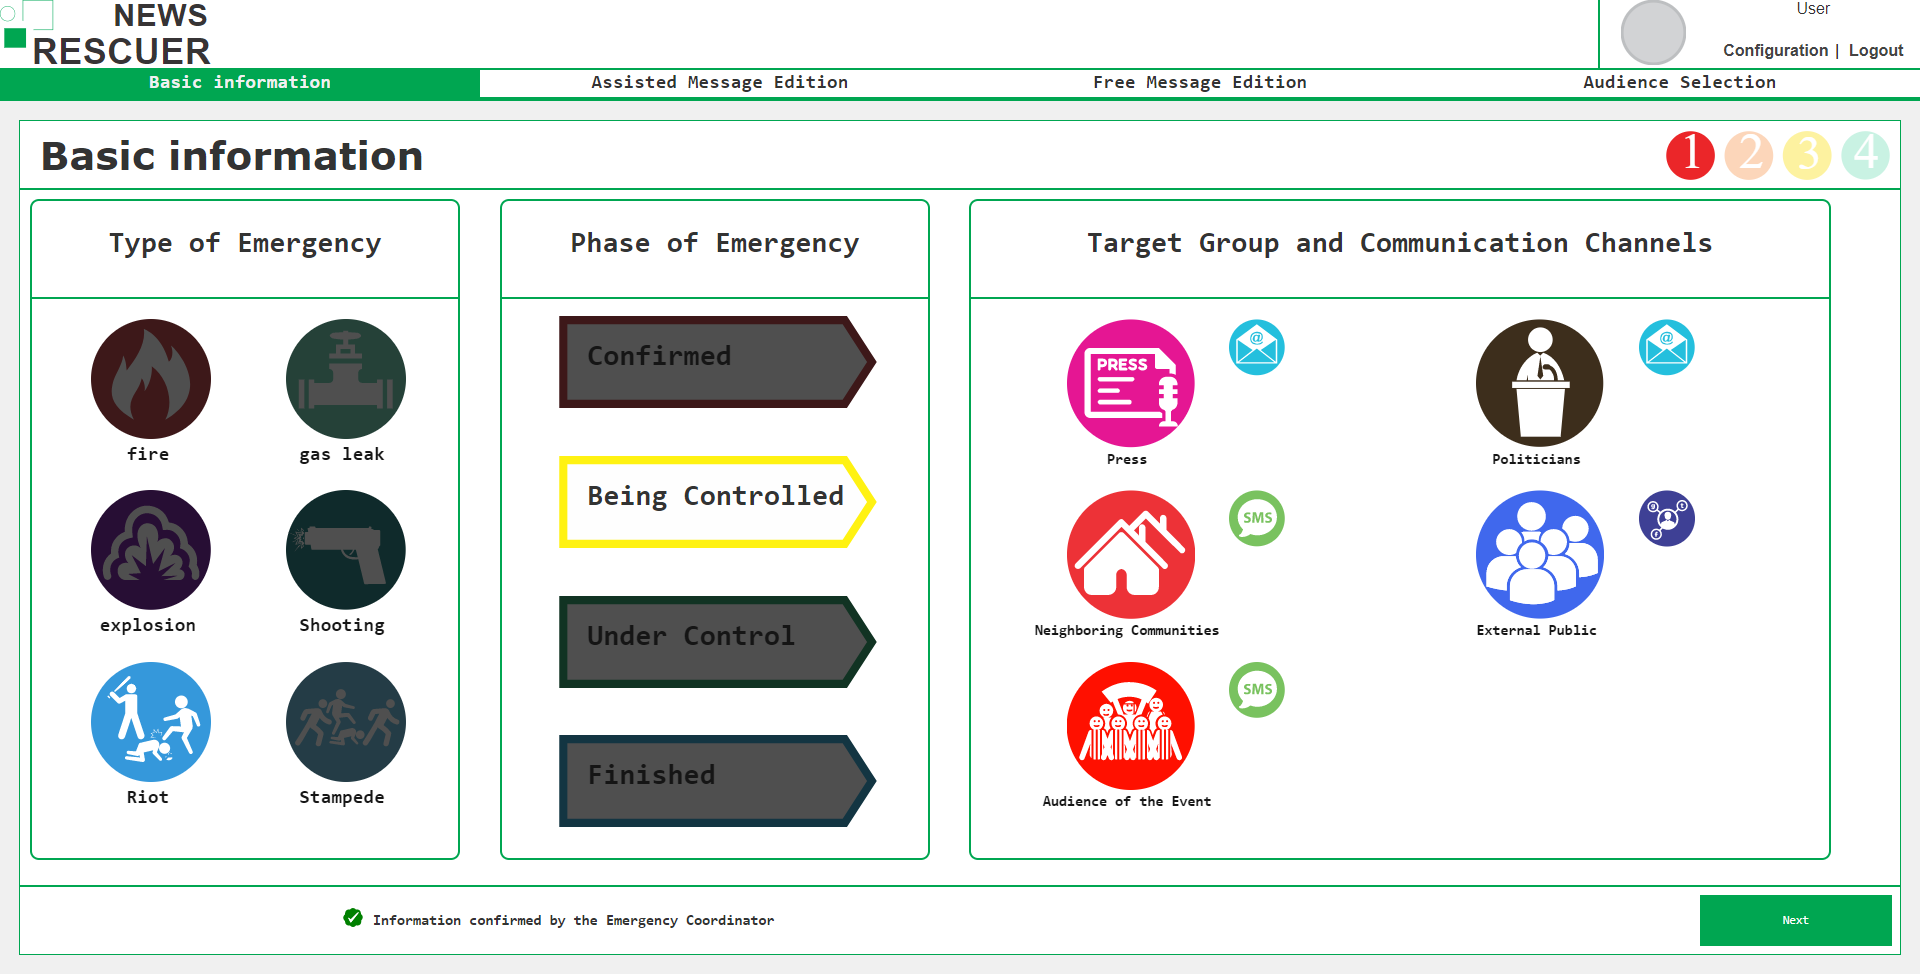
\includegraphics[width=0.85\linewidth]{images/DemoLinz1.png}
\label{demoStadium1}
}
\quad %espaco separador
\subfloat[Assisted Message Edition screen configured to build a public communication informing the occurrence episode of riot inside of the stadium]{
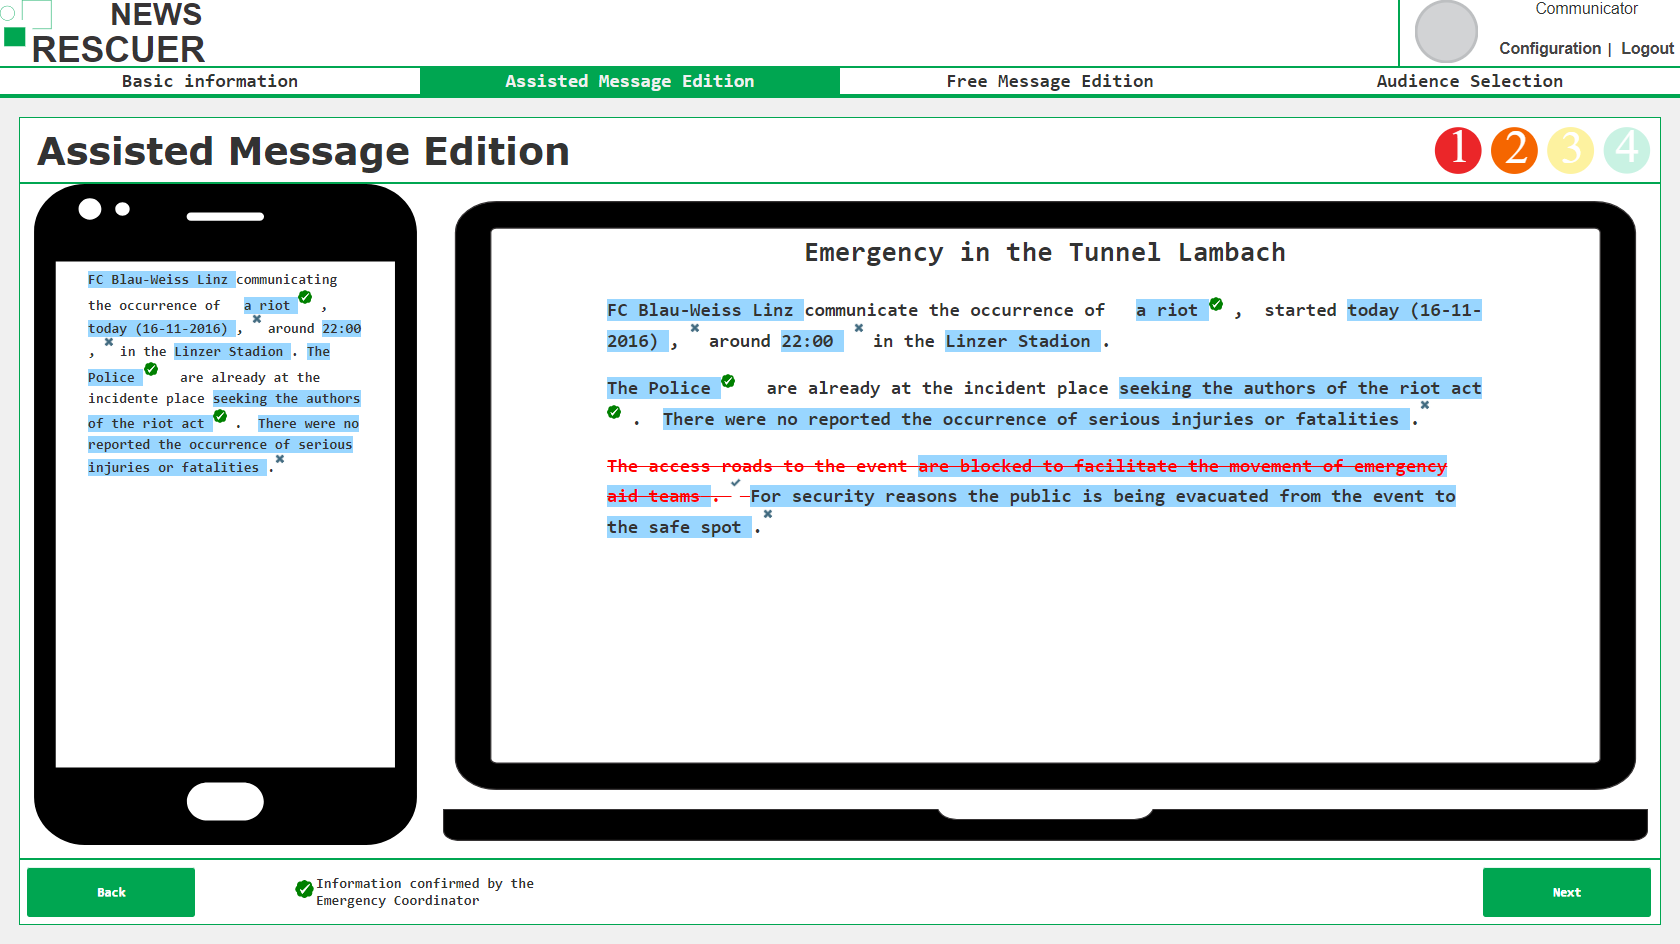
\includegraphics[width=0.85\linewidth]{images/DemoLinz2.png}
\label{demoStadium2}
}
\caption{RESCUER News configured for the demonstration at Stadion der Stadt Linz}
\label{demoStadium}
\end{figure*}

The event audience had the possibility to install and was encourage to use the RESCUER MCS  in order to know the proposal. In the other side, the event organisation was presented to RESCUER ERTK and had the opportunity to use RESCUER News to simulate sending public communication in different phases of an emergency. 

Figure \ref{demoStadium} presents RESCUER News configured to this demonstration. In Figure \ref{demoStadium1} we can see the Basic Information screen. In this screen we define the type of emergencies (a fire, a gas leakage, an explosion, a shootout, event of vandalism or a stampede (mass exodus)) that the system as enable to provide emergency public communications templates. We can also look the public audience available to receive public communication and each communication to possibility this. 


\begin{table*}[t]
\scalefont{0.6}
\centering
\caption{Analysis of the information contained in the template of a riot (incident type) being controlled (emergency phase) in a RESCUER Project demonstration at the Stadion der Stadt Linz}
\label{LinzInformationTable}
\begin{tabular}{cccccc}
\hline
Information & Value & \begin{tabular}[c]{@{}c@{}}Emergency State \\ Behaviour\end{tabular} & \begin{tabular}[c]{@{}c@{}}Exclusive for\\ Emergency Type\end{tabular} & \begin{tabular}[c]{@{}c@{}}Exclusive for\\ Stakeholder\end{tabular} & Removable \\ \hline
Communicator & \begin{tabular}[c]{@{}c@{}}FC Blau-Weiss\\ Linz\end{tabular} & Direct Association & -- & -- & Mandatory \\
Incident Type & a riot & \begin{tabular}[c]{@{}c@{}}Indirect Association\\ (incident type)\end{tabular} & Fire &  & Mandatory \\
Occurence Date & \begin{tabular}[c]{@{}c@{}}today\\ (16-11-2016)\end{tabular} & Direct Association & -- & -- & Mandatory \\
Occurence Time & 22:00 & Direct Association & -- & -- & Mandatory \\
Incident Place & Linzer Stadion & Direct Association & -- & -- & Mandatory \\
Response Team & The Police & \begin{tabular}[c]{@{}c@{}}Indirect Association\\ (incident type)\end{tabular} & \begin{tabular}[c]{@{}c@{}}Riot, Shooting\\ and Stampede\end{tabular} & -- & Mandatory \\
Response Action & \begin{tabular}[c]{@{}c@{}}seeking the authors of\\ the riot act\end{tabular} & \begin{tabular}[c]{@{}c@{}}Indirect Association\\ (incident type)\end{tabular} & Riot & -- & Mandatory \\
Injured People & \begin{tabular}[c]{@{}c@{}}There were no reported \\ the occurrence of serious \\ injuries or fatalities\end{tabular} & \begin{tabular}[c]{@{}c@{}}Based on the occurrence\\ (or not) of a fact\\ (injured people)\end{tabular} & -- & -- & Optional \\
\multicolumn{1}{l}{Roadblock} & \multicolumn{1}{l}{\begin{tabular}[c]{@{}l@{}}The access roads to the\\ event are blocked to \\ facilitate the movement \\ of emergency aid teams\end{tabular}} & \begin{tabular}[c]{@{}c@{}}Based on the occurrence\\ (or not) of a fact\\ (roadblock)\end{tabular} & -- & -- & Optional \\
Evacuation & \begin{tabular}[c]{@{}c@{}}For security reasons the \\ public is being \\ evacuated from the event\\ to the safe spot\end{tabular} & \begin{tabular}[c]{@{}c@{}}Based on the occurrence\\ (or not) of a fact\\ (roadblock)\end{tabular} & -- & -- & Optional
\end{tabular} 
\end{table*}

In the Figure \ref{demoStadium2}  we present the Assisted Message Editing interface configured with a template specified for the occurrence of a riot emergency in the phase that the emergency is "being controlled". On this public communication is informed that the Police (response team) is seeking the authors of the riot act. Was also informed that this incident does not cause injuries or fatalities, by then, however the event audience needed to be evacuated from the stadium, preventively. Table \ref{LinzInformationTable} presents the information contained in each sentence of this model, explaining in details the following characteristics: the type of information; its value; the emergency state behaviour that this information assumes; restriction by the type of emergency or by the type of stakeholder and if this sentence can be removable of this model. 



\section{Lambach Tunnel Emergency Simulation}

\begin{figure*}[!ht]
\centering
\subfloat[Basic information screen configured to the simulation in the Lambach Tunnel]{
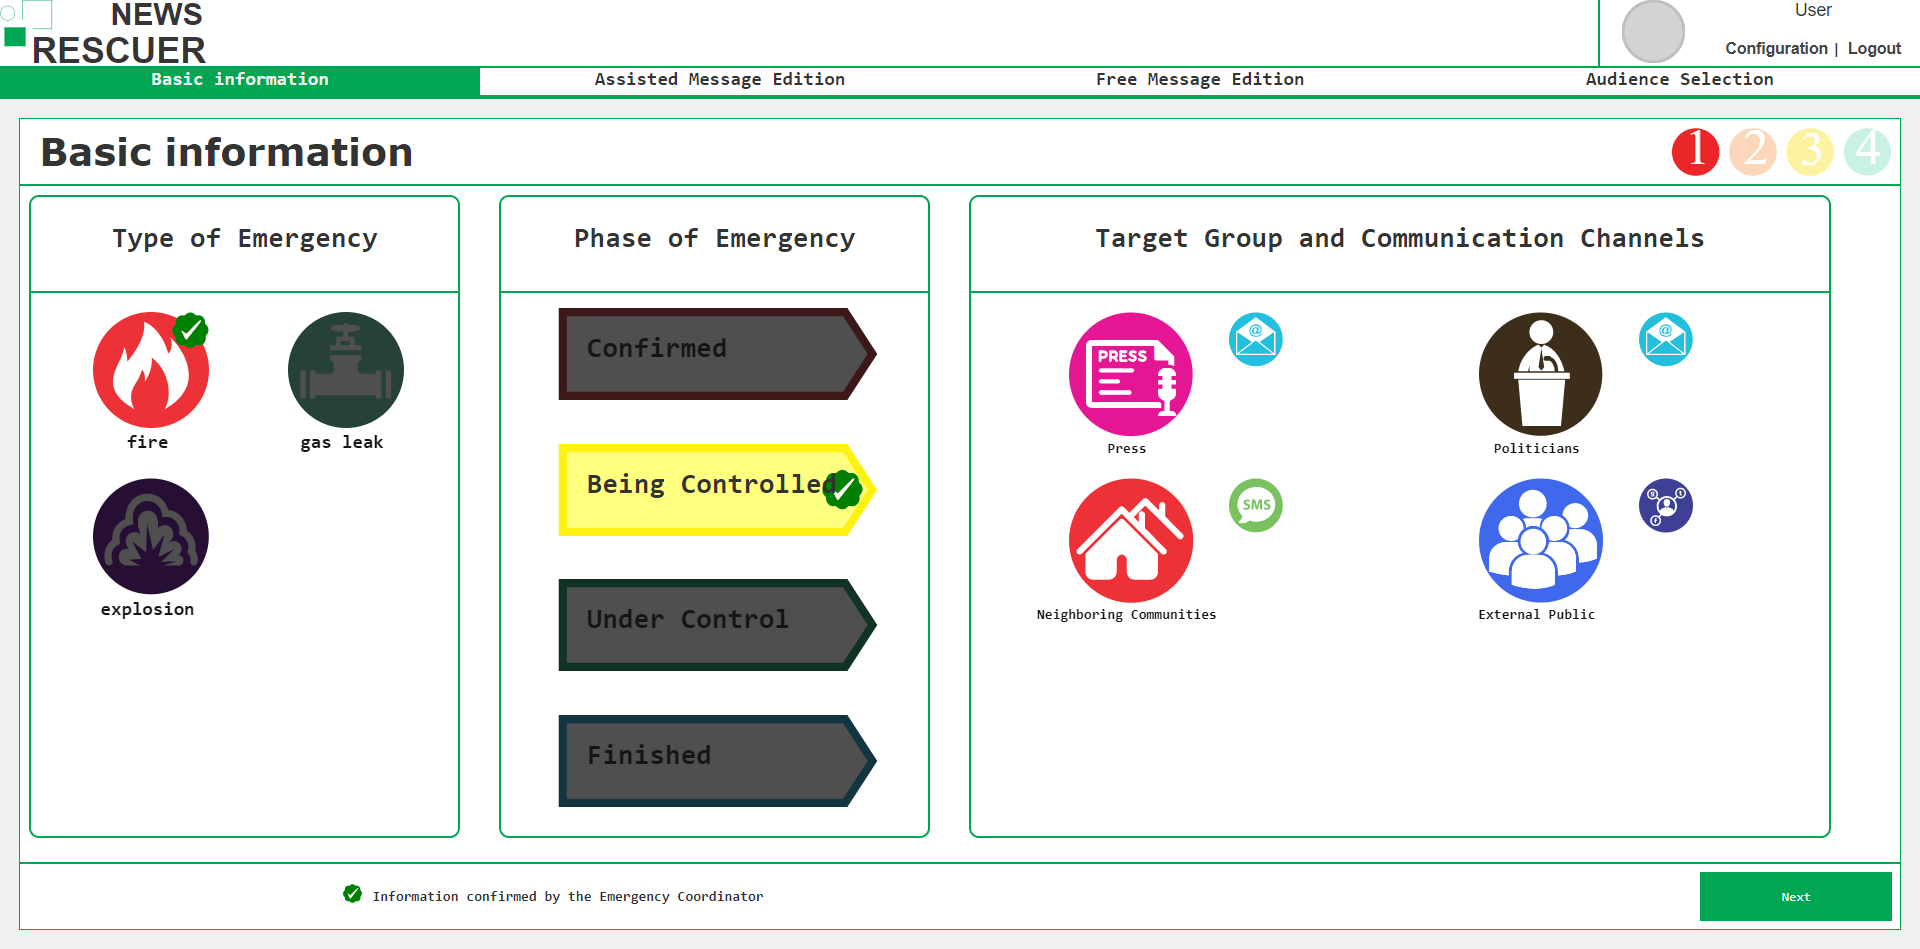
\includegraphics[width=0.75\linewidth]{images/DemoLambach1.png}
\label{demoLambach1}
}
\quad %espaco separador
\subfloat[Assisted Message Edition screen configured to build a public communication informing the occurrence of a fire inside of a tunnel]{
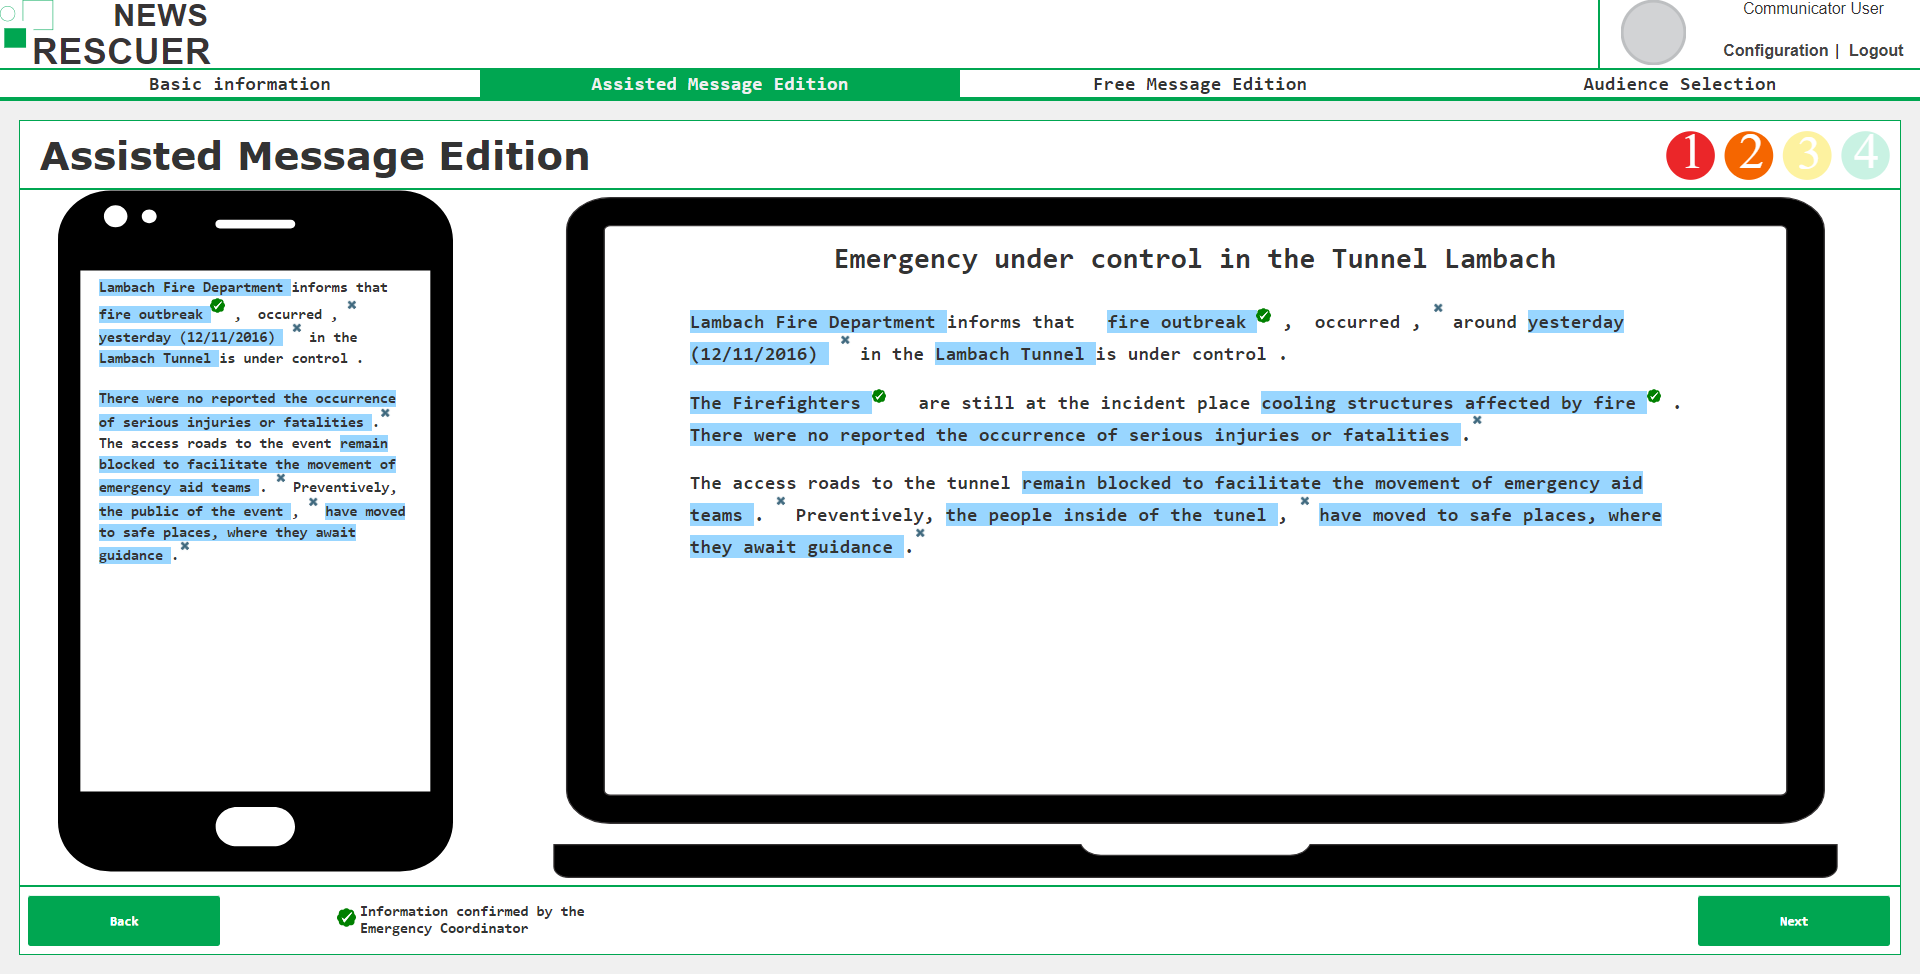
\includegraphics[width=0.85\linewidth]{images/DemoLambach2.png}
\label{demoLambach2}
}
\caption{RESCUER News configured for a simulation of a car accident inside of Lambach Tunnel}
\label{demoLambach}
\end{figure*}

This emergency simulation was conducted in a still unopened tunnel near the town of Lambach,
close to Linz, Austria. The simulated incident was a car accident in the tunnel, in which 3 vehicles were involved. One of them was represented to be on fire, with smoke in the tunnel represented by cold smoke.

This simulation involved ninety people, including public authorities, firefighters, police, rescuer teams and tunnel administration. Five of this people was in the Command and Control Centre, where they can monitor the emergencythrough RESCUER ERTK and use Rescuer News to send public communications.

In Figure \ref{demoLambach1} we present the Rescuer News basic information screen configured for this simulation. The types of incidents available for the Lambach Simulation were: a fire, gas leakage and explosion. We provided templates for 4 phases of the emergency (confirmed, being controlled, under control and finished). The target audiences configured to send public communications and the communication channel to dispatch for each of them as the following: press (email), politicians (email), neighboring communities (sms) and external public (the social networks Twitter and Facebook).

\begin{table*}[t]
\scalefont{0.6}
\centering
\caption{Analysis of the information contained in the template of a fire (incident type) under control (emergency phase) in the Lambach Tunnel simulation}
\label{lambachInformationTable}
\begin{tabular}{@{}lccccc@{}}
\toprule
\textbf{Information} & \textbf{Value} & \begin{tabular}[c]{@{}c@{}}Emergency State\\ Behaviour\end{tabular} & \begin{tabular}[c]{@{}c@{}}Exclusive for\\ Emergency Type\end{tabular} & \begin{tabular}[c]{@{}c@{}}Exclusive for\\ Stakeholder\end{tabular} & Removable \\ \midrule
Communicator & \begin{tabular}[c]{@{}c@{}}Lambach\\ Fire Department\end{tabular} & -- & -- & -- & Mandatory \\
Incident Type & Fire & Direct Association &  &  & Mandatory \\
Incident Description & fire outbreak & \begin{tabular}[c]{@{}c@{}}Indirect Association\\ (incident type)\end{tabular} & Fire & -- & Mandatory \\
Occurrence Time & \begin{tabular}[c]{@{}c@{}}yesterday\\ (12/11/2016)\end{tabular} & Direct Association & -- & -- & Mandatory \\
Incident Place & Lambach Tunnel & Direct Association & -- & -- & Mandatory \\
Response Team & The Firefighters & \begin{tabular}[c]{@{}c@{}}Indirect Association\\ (incident type)\end{tabular} & \begin{tabular}[c]{@{}c@{}}Fire and\\ Gas Leakage\end{tabular} & -- & Mandatory \\
Response Action & \begin{tabular}[c]{@{}c@{}}cooling structures \\ affected by fire\end{tabular} & \begin{tabular}[c]{@{}c@{}}Indirect Association \\ (incident type)\end{tabular} & Fire & -- & Mandatory \\
Road Block & \begin{tabular}[c]{@{}c@{}}remain blocked to \\ facilitate the movement\\ of emergency aid teams\end{tabular} & \begin{tabular}[c]{@{}c@{}}Based on the occurrence \\ (or not) of a fact \\ (road block)\end{tabular} & -- & -- & Optional \\
Evacuation Group & \begin{tabular}[c]{@{}c@{}}the people inside \\ of the tunnel\end{tabular} & \begin{tabular}[c]{@{}c@{}}Based on the occurrence\\ (or not) of a fact \\ (evacuation)\end{tabular} & -- & -- & Optional \\
Evacuation Action & \begin{tabular}[c]{@{}c@{}}have moved to \\ safe places, where \\ they await guidance\end{tabular} & \begin{tabular}[c]{@{}c@{}}Based on the occurrence\\ (or not) of a fact\\  (evacuation)\end{tabular} & -- & -- & Optional
\end{tabular}
\end{table*}


Figure \ref{demoLambach2} present the Rescuer News Assisted Message Edition screen configured with a template for an incident type fire during the phase that the incident is "under control". On this public communication is informed that the Firefighters (response team) is cooling the structures affected by the fire (response action). In addition, it was informed that the emergency does not cause injuries or fatalities, however, it was necessary to maintain the roadblocks and evacuate the people inside of the tunnel. Table \ref{lambachInformationTable} explains in details the characteristic of each information presented in this phase template. 


\section{Cama\c{c}ari Industrial Complex simulation}

Our last simulation happened in the Industrial Complex of Cama\c{c}ari. We simulated the occurrence of a fire in an industrial plant. Involved people act during a real emergency or are affected by the consequences of an emergency. The participants were divided into emergency managers, people who work as support force (doctors, security guards, and police officers), workforce (firefighters and company brigade) and neighbouring communities. 

In Figure \ref{demoPolo} we present the Rescuer News configured to the scenario of the Industrial park. 

\begin{figure*}[h]
\centering
\subfloat[Basic information screen configured to the simulation in the Cama\c{c}ari Industrial Complex]{
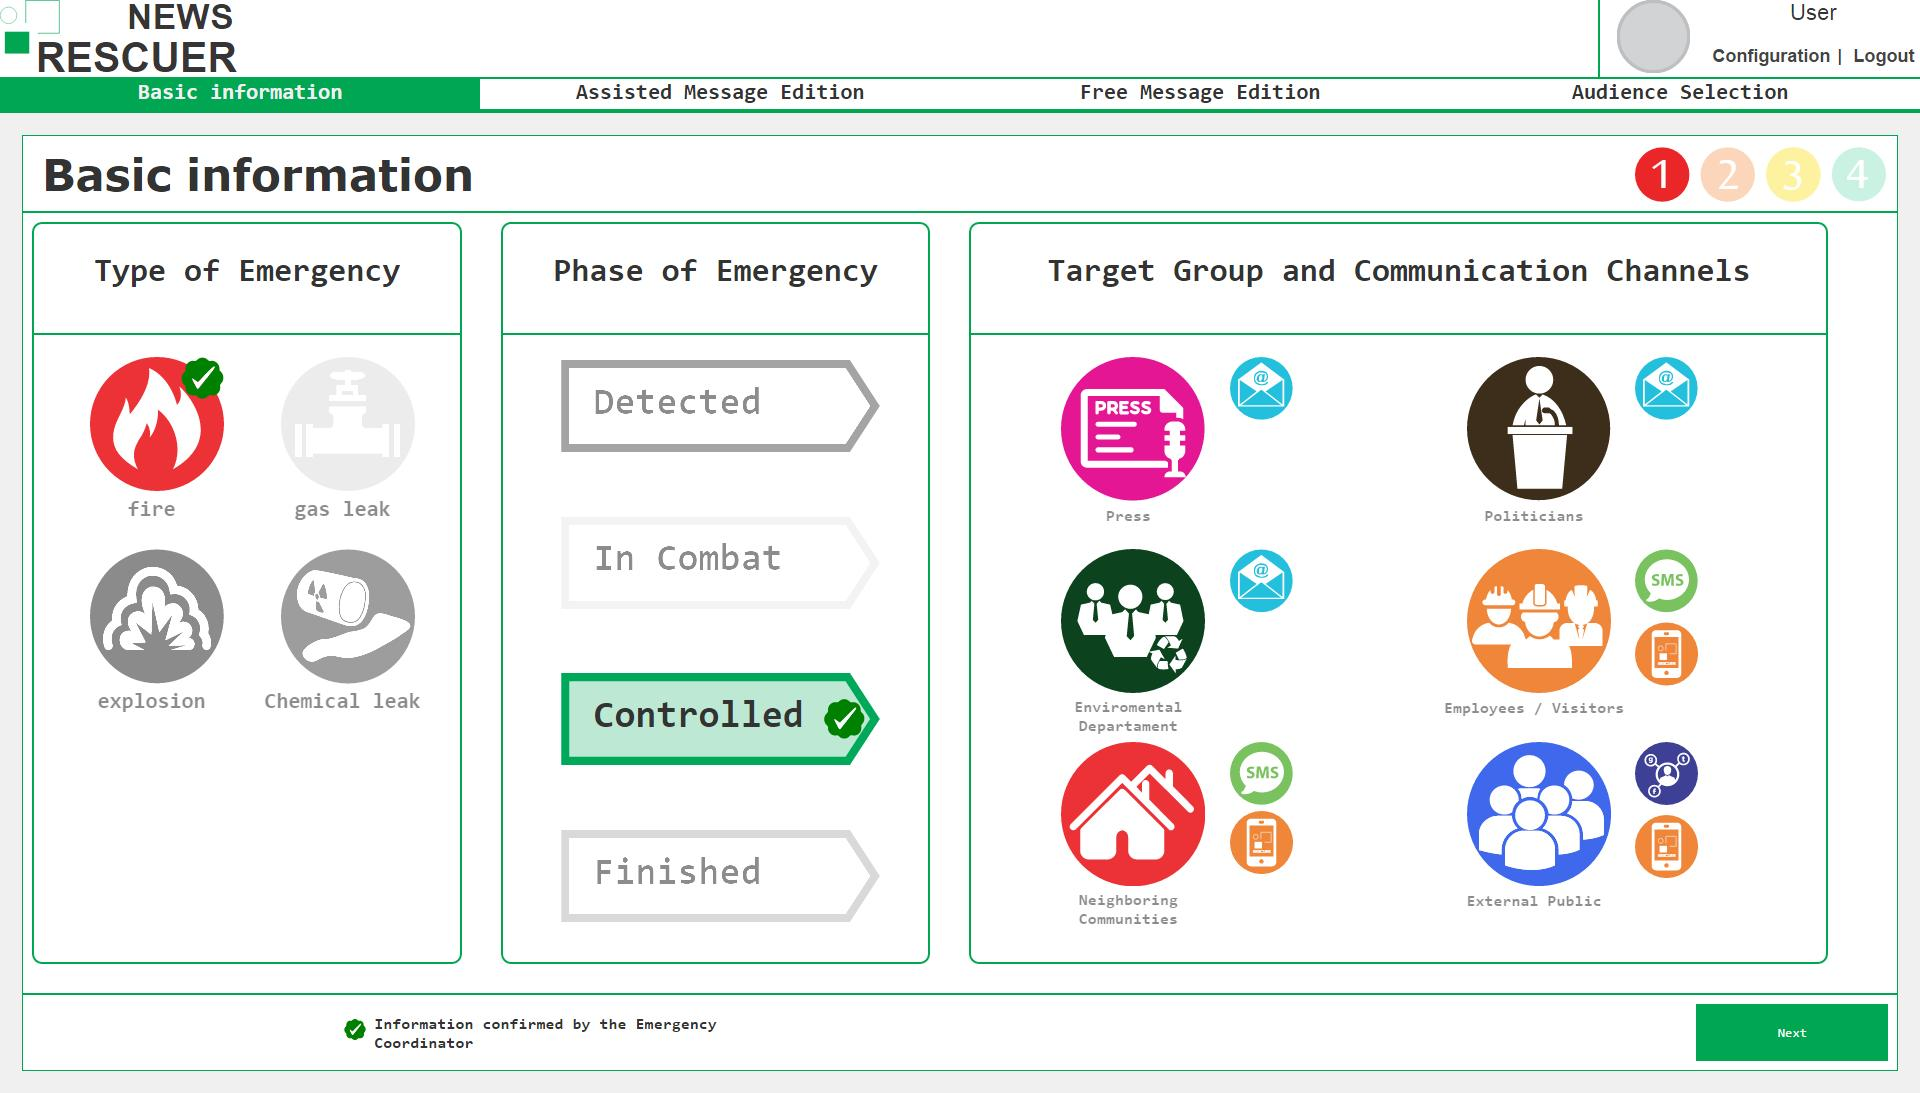
\includegraphics[width=0.85\linewidth]{images/DemoPolo1.jpg}
\label{demoPolo1}
}
\quad %espaco separador
\subfloat[Assisted Message Edition screen configured to build a public communication informing the occurrence of a gas leak in a industrial complex]{
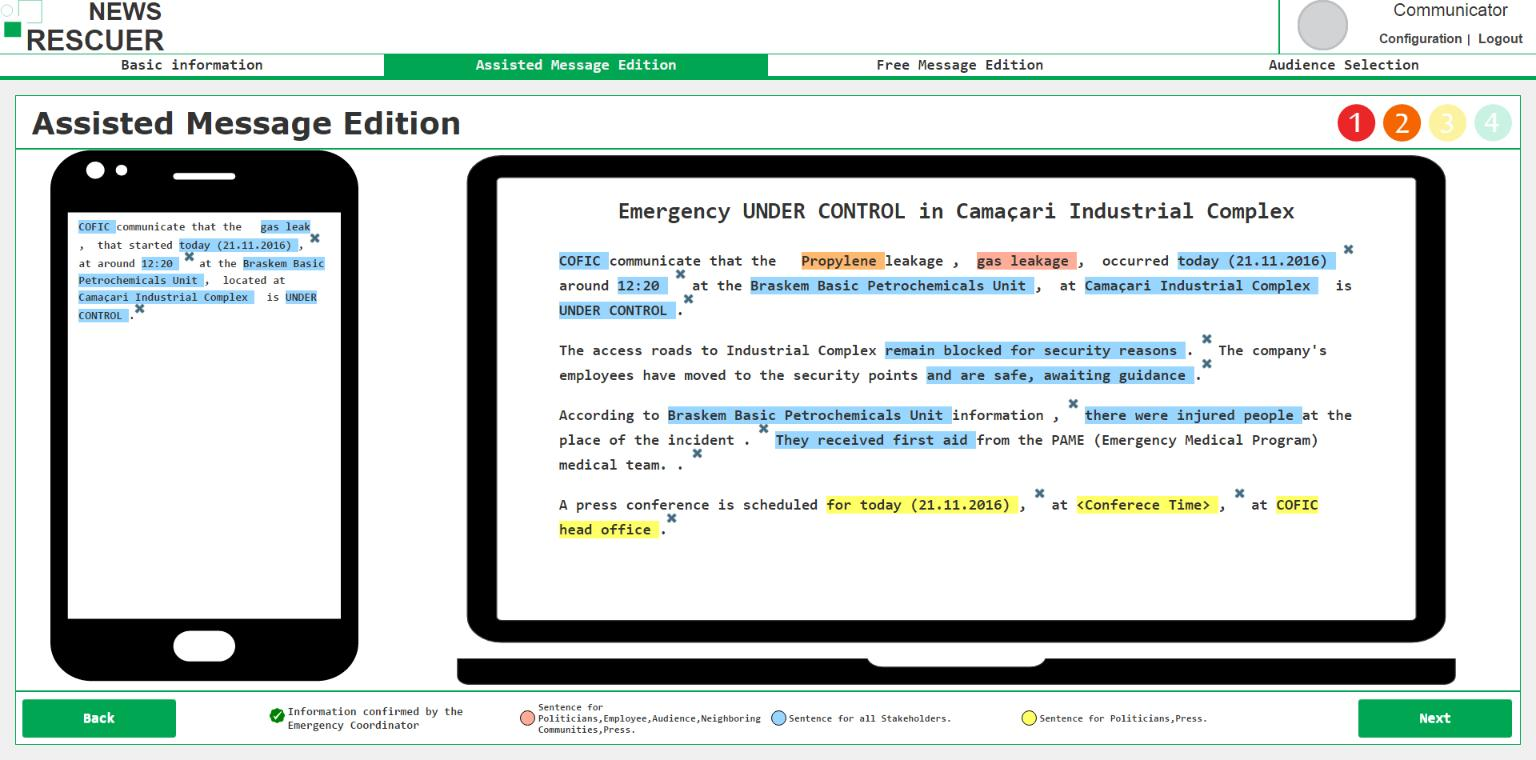
\includegraphics[width=0.85\linewidth]{images/DemoPolo2.jpg}
\label{demoPolo2}
}
\caption{RESCUER News configured for the Cama\c{c}ari Industrial Park simulation}
\label{demoPolo}
\end{figure*}

For this simulation, we configure the Rescuer News to work with incidents like a fire, a gas leakage, an explosion and a chemical leak. We build communication models for 4 emergency phases (detected, in combat, controlled, finished). The stakeholders and the communication channel selected for this scenario was the following: Press, Politicians and Environmental department by email; Employees, company visitors and neighbouring communities by SMS and RESCUER MCS; and External Public by posts in Social Network and Rescuer MCS. The Figure \ref{demoPolo1} present the Basic Information screen of the RESCUER News configured with this information.


The Figure \ref{demoPolo2} presents the Assisted Message Edition screen with a public communication model informing the control of an incident of gas leakage (propylene leakage). In addition, this public release informs the consequences of this incident like roadblocks, evacuation, and occurrence of injured people. In special, an information about a press conference will be sent exclusively in the public release addressed for politicians and press (sentences exclusive for specifics stakeholders). Table \ref{camacariInformationTable} present, in details, the sentences of this public communication model, explaining each characteristic and restrictions of them.


% Please add the following required packages to your document preamble:
% \usepackage{booktabs}
\begin{table*}[t]
\scalefont{0.60}
\centering
\caption{Analysis of the information contained in the template of a gas leakage (incident type) under control (emergency phase) in the Cama\c{c}ari Industrial Complex}
\label{camacariInformationTable}
\begin{tabular}{@{}cccccc@{}}
\toprule
Information & Value & \begin{tabular}[c]{@{}c@{}}Emergency State \\ Behaviour\end{tabular} & \begin{tabular}[c]{@{}c@{}}Exclusive for\\ Emergency Type\end{tabular} & \begin{tabular}[c]{@{}c@{}}Exclusive for\\ Stakeholder\end{tabular} & Removable \\ \midrule
Communicator & COFIC & Direct Association & -- & -- & Mandatory \\
\begin{tabular}[c]{@{}c@{}}Incident Type\\ Description\end{tabular} & Propylene & \begin{tabular}[c]{@{}c@{}}Indirect Association\\ (incident type)\end{tabular} & Gas Leakage & \begin{tabular}[c]{@{}c@{}}Environmental\\ Department\end{tabular} & Mandatory \\
\begin{tabular}[c]{@{}c@{}}Incident Type\\ Description\end{tabular} & gas leakage & \begin{tabular}[c]{@{}c@{}}Indirect Association\\ (incident type)\end{tabular} & Gas Leakage & \begin{tabular}[c]{@{}c@{}}Other\\ Stakeholders\end{tabular} & Mandatory \\
Occurrence Date & \begin{tabular}[c]{@{}c@{}}today\\ (21-11-2016)\end{tabular} & Direct Association & -- & -- & Mandatory \\
Occurrence Time & 12:20 & Direct Association & -- & -- & Mandatory \\
\begin{tabular}[c]{@{}c@{}}Affected \\ Company\end{tabular} & \begin{tabular}[c]{@{}c@{}}Braskem Basic \\ Petrochemical Unit\end{tabular} & Direct Association & -- & -- & Mandatory \\
\begin{tabular}[c]{@{}c@{}}Affected\\ Location\end{tabular} & \begin{tabular}[c]{@{}c@{}}Cama\c{c}ari Industrial\\ Complex\end{tabular} & Direct Association & -- & -- & Mandatory \\
Roadblock & \begin{tabular}[c]{@{}c@{}}remain blocked for\\ security reasons\end{tabular} & \begin{tabular}[c]{@{}c@{}}Based on the occurrence\\ (or not) of a fact\\ (injured people)\end{tabular} & -- & -- & Optional \\
Evacuation & \begin{tabular}[c]{@{}c@{}}and are safe, \\ awaiting guidance\end{tabular} & \begin{tabular}[c]{@{}c@{}}Based on the occurrence\\ (or not) of a fact\\ (injured people)\end{tabular} & -- & -- & Optional \\
Injured People & \begin{tabular}[c]{@{}c@{}}there were \\ injured people\end{tabular} & \begin{tabular}[c]{@{}c@{}}Based on the occurrence\\ (or not) of a fact\\ (injured people)\end{tabular} & -- & -- & Optional \\
\begin{tabular}[c]{@{}c@{}}Injured People\\ Response Action\end{tabular} & They received first aid & \begin{tabular}[c]{@{}c@{}}Based on the occurrence\\ (or not) of a fact\\ (injured people)\end{tabular} & -- & -- & Optional \\
\begin{tabular}[c]{@{}c@{}}Press \\ Conference\\ Date\end{tabular} & for today (21.11.2016) & Direct Association & -- & \begin{tabular}[c]{@{}c@{}}Press and\\ Politicians\end{tabular} & Optional \\
\begin{tabular}[c]{@{}c@{}}Press\\ Conference\\ Time\end{tabular} & \textless{}Conference Time\textgreater{} & Direct Association & -- & \begin{tabular}[c]{@{}c@{}}Press and\\ Politicians\end{tabular} & Optional \\
\begin{tabular}[c]{@{}c@{}}Press\\ Conference\\ Place\end{tabular} & \begin{tabular}[c]{@{}c@{}}COFIC \\ head office\end{tabular} & Direct Association & -- & \begin{tabular}[c]{@{}c@{}}Press and\\ Politicians\end{tabular} & Optional \\ \bottomrule
\end{tabular}
\end{table*}


\section{Discussion}

\textcolor{red}{ToDo Jorge: Apresentar o feedback do túnel lambach e falar um pouco sobre o feedback do polo incluindo o interesse em utilizar a solução }

\textcolor{red}{Sinto falta de uma seção de discussão dos experimentos realizados, avaliando se funcionou ou nao, o que os usuarios acharam ou nao. Além disso, a instanciacao do modelo precisaria ficar mais evidente que isso é o que foi feito nessa prova de conceito. Linkar melhor o modelo com os resultados dos experimentos.}